\documentclass[border=10pt]{standalone}
\usepackage[svgnames]{xcolor}
\usepackage{amsmath}
\usepackage{pgfplots}
\pgfplotsset{compat=newest}
\usepackage[sfdefault]{FiraSans}
\usepackage{FiraMono}
\renewcommand*\familydefault{\sfdefault}
\begin{document}
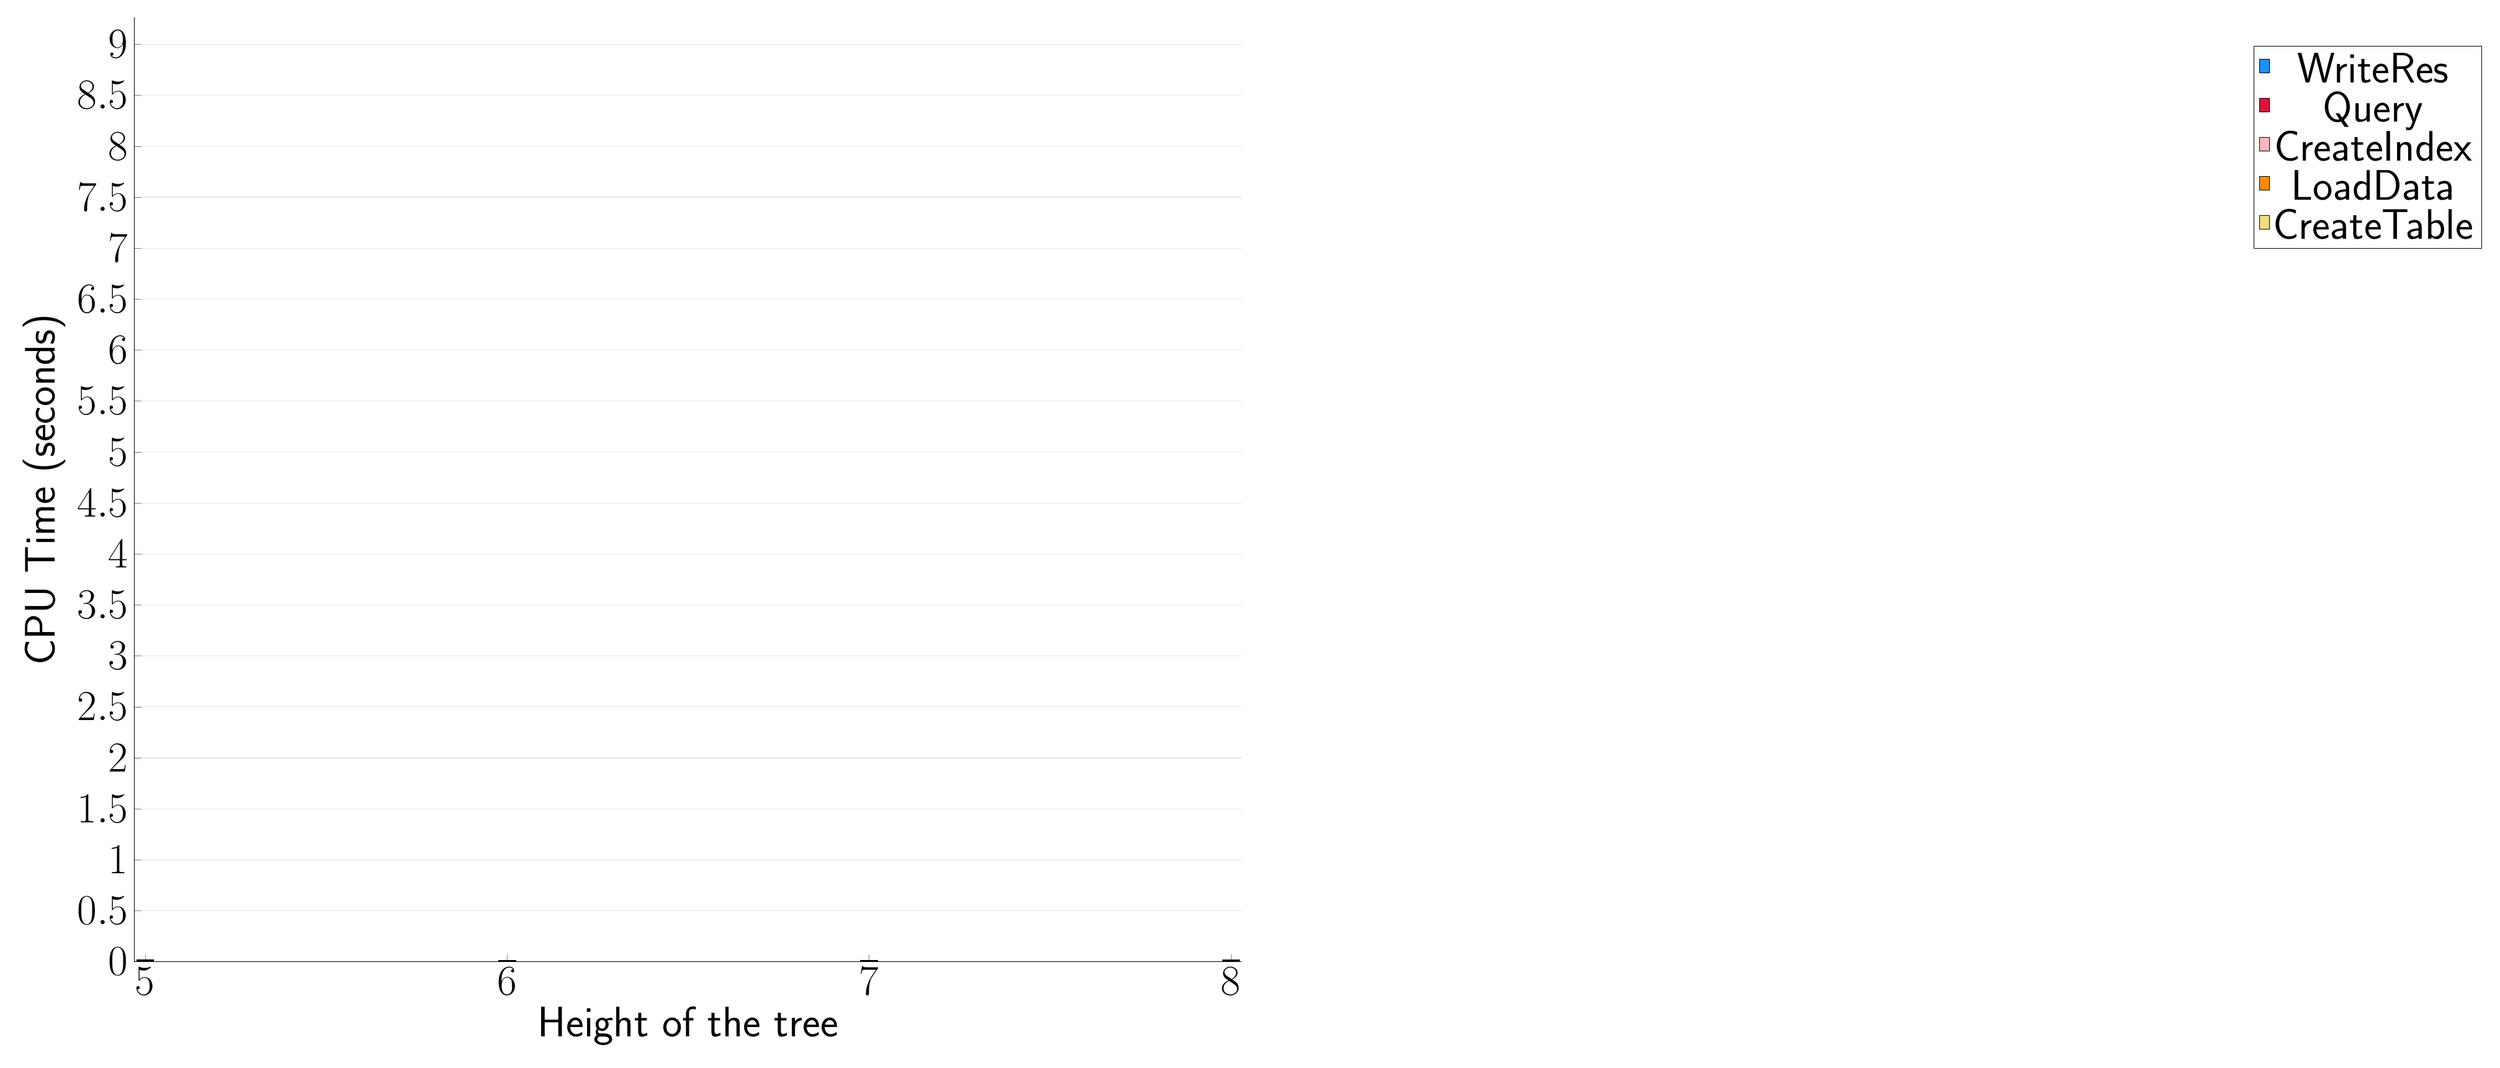
\begin{tikzpicture}
\begin{axis}[
   ybar stacked,
   width=2\textwidth,
   bar width=0.35cm,
   ymajorgrids, tick align=inside,
   major grid style={draw=gray!20},
   xtick=data,
   ymin=0, ymax=9.263333335518837,
   axis x line*=bottom,
   axis y line*=left,
   enlarge x limits=0.01,
   legend style={
       at={(2.12, 0.97)},
       anchor=north east,
       legend columns=1,
       font=\Huge,
   },
   ylabel={CPU Time (seconds)},
   xlabel={Height of the tree},
   label style={font=\Huge},
   tick label style={font=\Huge},
]
\addlegendimage{fill=DodgerBlue, draw=black, line width=0.2pt}
\addlegendentry{WriteRes}
\addlegendimage{fill=Crimson, draw=black, line width=0.2pt}
\addlegendentry{Query}
\addlegendimage{fill=LightPink, draw=black, line width=0.2pt}
\addlegendentry{CreateIndex}
\addlegendimage{fill=DarkOrange, draw=black, line width=0.2pt}
\addlegendentry{LoadData}
\addlegendimage{fill=LightGoldenrod, draw=black, line width=0.2pt}
\addlegendentry{CreateTable}
\addplot +[fill=LightGoldenrod, draw=black, line width=0.2pt] coordinates {
(5, 0.006666666666666672)
(6, 0.009999999999999986)
(7, 0.006666666666666674)
(7, 0.006666666666666674)
(7, 0.009999999999999972)
(8, 0.003333333333333337)
(8, 0.006666666666666672)
(8, 0.010000000000000005)
};
\addplot +[fill=DarkOrange, draw=black, line width=0.2pt] coordinates {
(5, 0.006666666666666669)
(6, 0.003333333333333337)
(7, 0.0)
(7, 0.0)
(7, 0.0)
(8, 0.003333333333333337)
(8, 0.003333333333333337)
(8, 0.0)
};
\addplot +[fill=LightPink, draw=black, line width=0.2pt] coordinates {
(5, 0.006666666666666668)
(6, 0.0)
(7, 0.0)
(7, 0.0)
(7, 0.0)
(8, 0.0033333333333333344)
(8, 0.0)
(8, 0.006666666666666652)
};
\addplot +[fill=Crimson, draw=black, line width=0.2pt] coordinates {
(5, 0.0)
(6, 0.0)
(7, 0.0)
(7, 0.0033333333333333375)
(7, 0.0)
(8, 0.0)
(8, 0.0)
(8, 0.0)
};
\addplot +[fill=DodgerBlue, draw=black, line width=0.2pt] coordinates {
(5, 0.003333333333333336)
(6, 0.0)
(7, 0.006666666666666655)
(7, 0.006666666666666637)
(7, 0.003333333333333337)
(8, 0.009999999999999993)
(8, 0.006666666666666672)
(8, 0.003333333333333336)
};
\end{axis}
\end{tikzpicture}

\end{document}
